% Bien dich tren Overleaf bang pdfLaTeX; tep nguon UTF-8.
% Nguon phuong phap: kaggle_ablation_u4_all_noise_512_100ep.ipynb.
% Hinh 1a/1b/1c: output/imgs/1a.png, 1b.png, 1c.png (so do doc tu Colab).
% Hinh 2: output/imgs/2.png, tu notebooks/colab_draw_fig02_architecture.ipynb.
% Hinh 3: scripts/build_paper_figures.py.
% Khung hinh ket qua va cac o -- de bo sung sau; tach giao thuc 512/3600.
\documentclass[conference]{IEEEtran}
\IEEEoverridecommandlockouts
\usepackage[utf8]{vietnam}
\usepackage{cite}
\usepackage{amsmath,amssymb,amsfonts}
\usepackage{algorithmic}
\usepackage{graphicx}
\graphicspath{{output/imgs/}{output/pdf/figures/}{figures/}}
% Giu dinh dang caption IEEE; tach Hinh 1 thanh ba float lien tiep 1a/1b/1c.
\usepackage[caption=false,font=footnotesize]{subfig}
\usepackage{textcomp}
\usepackage{xcolor}
\usepackage{booktabs}
\usepackage{array}
\usepackage[hidelinks]{hyperref}

\renewcommand{\abstractname}{Tóm tắt}
\renewcommand{\IEEEkeywordsname}{Từ khóa}
\renewcommand{\figurename}{Hình}
\renewcommand{\tablename}{Bảng}
\renewcommand{\refname}{Tài liệu tham khảo}
\pdfstringdefDisableCommands{\def\ecircumflex{e}}
\AtBeginDocument{\renewcommand{\refname}{Tài liệu tham khảo}}
\renewcommand{\algorithmicrequire}{\textbf{Đầu vào:}}
\renewcommand{\algorithmicensure}{\textbf{Đầu ra:}}
\renewcommand{\algorithmicfor}{\textbf{với}}
\renewcommand{\algorithmicdo}{\textbf{thực hiện}}
\renewcommand{\algorithmicendfor}{\textbf{kết thúc vòng lặp}}
\newcommand{\pending}{\textemdash}
\newcommand{\draftnote}[1]{\textit{[Bổ sung: #1]}}
\newcommand{\figplaceholder}[2]{%
  \fbox{\parbox[c][#1][c]{\dimexpr\linewidth-2\fboxsep-2\fboxrule\relax}{%
    \centering\small #2}}}
% Moi so do doc chiem mot cot; gioi han chieu cao de con cho caption.
% Hinh 1 dung truc tiep ba PNG hien co trong output/imgs/.
\newcommand{\systempanelinclude}[1]{%
  \includegraphics[width=\linewidth,height=0.83\textheight,keepaspectratio]{#1}}
\DeclareMathOperator{\Concat}{Concat}
\DeclareMathOperator{\Conv}{Conv1D}
\DeclareMathOperator{\IN}{IN}
\DeclareMathOperator{\ReLU}{ReLU}
\DeclareMathOperator{\SiLU}{SiLU}
\DeclareMathOperator{\softmax}{softmax}
\DeclareMathOperator{\STFT}{STFT}

\begin{document}

\title{Khử nhiễu tín hiệu ECG bằng mô hình khuếch tán có điều kiện kết hợp HNF--FiLM 1D U-Net}

\author{\IEEEauthorblockN{Vũ Duy Hưng}
\IEEEauthorblockA{\textit{Khoa Công nghệ Thông tin} \\
\textit{Trường Đại học Công Thương TP.HCM (HUIT)}\\
TP. Hồ Chí Minh, Việt Nam \\
2001230325@huit.edu.vn}}

\maketitle

\begin{abstract}
Tín hiệu điện tâm đồ (ECG) dễ bị ảnh hưởng bởi nhiễu trôi đường nền, chuyển động điện cực và hoạt động cơ trong quá trình thu nhận. Những thành phần này có thể che khuất đặc trưng của tín hiệu, trong khi quá trình lọc quá mức có thể làm biến dạng dạng sóng cần phục hồi. Nghiên cứu này đề xuất phương pháp khử nhiễu ECG một đạo trình dựa trên mô hình khuếch tán có điều kiện, với mạng dự đoán nhiễu là một biến thể 1D U-Net. Kiến trúc tích hợp khối lọc chuẩn hóa một phần HNF để trích xuất đặc trưng đa tỉ lệ, điều chế FiLM theo mức khuếch tán và self-attention tại bottleneck. Mục tiêu huấn luyện kết hợp sai số dự đoán nhiễu trong miền thời gian với sai số biên độ STFT tương đối của ECG tái tạo, được điều chỉnh theo tỷ số tín hiệu trên nhiễu của quá trình khuếch tán. ECG tham chiếu lấy từ QT Database; các nguồn nhiễu lấy từ MIT-BIH Noise Stress Test Database. Một mô hình được huấn luyện trên các đoạn 512 điểm với bảy tổ hợp không rỗng của ba nguồn nhiễu, nhằm xử lý nhiều dạng nhiễu bằng cùng một bộ tham số. Đóng góp của từng thành phần kiến trúc được khảo sát qua năm biến thể U0--U4 dưới cùng giao thức dữ liệu và huấn luyện. Chất lượng phục hồi được đánh giá bằng sai số tín hiệu, mức cải thiện SNR, độ tương đồng dạng sóng và chi phí suy luận DDIM. \draftnote{các kết quả định lượng chính sau khi hoàn tất đánh giá thống nhất.}
\end{abstract}

\begin{IEEEkeywords}
ECG, khử nhiễu, khuếch tán có điều kiện, 1D U-Net, HNF, FiLM, DDIM.
\end{IEEEkeywords}

\section{Giới thiệu}
ECG biểu diễn hoạt động điện của tim theo thời gian và là nguồn dữ liệu quan trọng trong phân tích tín hiệu y sinh. Hình thái, biên độ và quan hệ thời gian giữa các thành phần P, QRS và T cung cấp thông tin cho các bước phân tích tiếp theo. Tuy nhiên, chất lượng bản ghi phụ thuộc vào điều kiện đo và dễ suy giảm bởi nhiễu trôi đường nền (baseline wander, BW), nhiễu chuyển động điện cực (electrode motion, EM) và nhiễu cơ (muscle artifact, MA). Các nguồn nhiễu này có đặc tính khác nhau và có thể đồng thời xuất hiện trong một bản ghi\cite{chiang2019,nstdb}.

Khử nhiễu ECG đòi hỏi cân bằng giữa mức độ loại bỏ nhiễu và mức độ duy trì tín hiệu gốc. Các bộ lọc truyền thống có ưu điểm về tính đơn giản và chi phí tính toán, nhưng hiệu quả phụ thuộc vào giả thiết về dải tần hoặc khả năng quan sát nguồn nhiễu tham chiếu\cite{thakor1991}. Khi đặc trưng nhiễu và ECG chồng lấn, việc triệt bỏ một thành phần theo tần số có thể đồng thời tác động đến tín hiệu mong muốn. Các phương pháp học sâu tiếp cận bài toán bằng cách học ánh xạ từ ECG nhiễu sang ECG tham chiếu, từ đó giảm phụ thuộc vào việc thiết kế bộ lọc thủ công\cite{chiang2019,deepfilter,fgdae}.

Mô hình khuếch tán cung cấp một cách tiếp cận khác: học quá trình khôi phục dữ liệu qua nhiều mức nhiễu Gaussian\cite{ddpm}. Khi bổ sung ECG quan sát làm điều kiện, quá trình phục hồi được định hướng theo đầu vào thay vì chỉ sinh tín hiệu từ phân phối chung. DeScoD-ECG đã khai thác mô hình khuếch tán có điều kiện cho khử nhiễu ECG\cite{descod}. Trong hướng tiếp cận này, mạng dự đoán nhiễu cần biểu diễn chi tiết cục bộ, ngữ cảnh thời gian và thông tin về mức khuếch tán. Chất lượng mạng và số lần gọi mạng trong quá trình lấy mẫu quyết định sự đánh đổi giữa độ chính xác và chi phí suy luận.

Nghiên cứu này xây dựng mạng HNF--FiLM 1D U-Net trong khung khuếch tán có điều kiện. Khối HNF kết hợp tích chập đa tỉ lệ với chuẩn hóa trên một phần số kênh; FiLM điều chế đặc trưng theo mức khuếch tán; self-attention được đặt ở biểu diễn đã giảm độ phân giải. Các thành phần được tích hợp nhằm hỗ trợ phục hồi ECG chịu nhiều loại nhiễu và được kiểm chứng bằng thí nghiệm loại bỏ thành phần. Các nội dung chính gồm:
\begin{itemize}
 \item Thiết kế mạng dự đoán nhiễu một chiều kết hợp HNF, FiLM và self-attention trong conditional DDPM.
 \item Xây dựng mục tiêu học kết hợp dự đoán nhiễu và sai số phổ tương đối, có trọng số để hạn chế ảnh hưởng của các mức khuếch tán có SNR thấp.
 \item Thiết lập giao thức một mô hình xử lý bảy tổ hợp BW/EM/MA và phép so sánh U0--U4 với cùng cặp dữ liệu, loss và ngân sách huấn luyện.
\end{itemize}
Phạm vi đánh giá của bài là chất lượng phục hồi tín hiệu. Khả năng bảo toàn chẩn đoán lâm sàng cần được kiểm chứng bằng các thí nghiệm chuyên biệt và không được suy ra chỉ từ chỉ số sai số tổng thể.

\section{Các nghiên cứu liên quan}
\subsection{Các phương pháp lọc truyền thống}
Lọc thích nghi sử dụng quan hệ giữa tín hiệu đầu vào và nguồn tham chiếu để ước lượng thành phần nhiễu. Thakor và Zhu\cite{thakor1991} nghiên cứu nhiều cấu trúc lọc cho các dạng nhiễu ECG khác nhau; khả năng cung cấp nguồn tham chiếu phù hợp là một yếu tố quan trọng của hướng tiếp cận này. Các phương pháp dựa trên biến đổi wavelet hoặc ước lượng đường nền khai thác phân rã đa độ phân giải để phân biệt thành phần cần giữ và cần loại bỏ. Romero và cộng sự\cite{bwcomparison} khảo sát các phương pháp loại bỏ BW, gợi mở việc lựa chọn thuật toán gắn với giao thức và đặc tính tín hiệu. Các phương pháp này là đối chứng hữu ích nhờ cơ chế xử lý rõ ràng, đồng thời đặt ra bài toán duy trì dạng sóng khi nhiễu và ECG có thành phần chồng lấn.

\subsection{Các mô hình học sâu cho khử nhiễu ECG}
Chiang và cộng sự\cite{chiang2019} sử dụng denoising autoencoder tích chập hoàn toàn để phục hồi ECG từ phiên bản có nhiễu. DeepFilter\cite{deepfilter} học bộ lọc BW từ dữ liệu, trong khi Fully-Gated Denoising Auto-Encoder\cite{fgdae} sử dụng cơ chế gating cho bài toán giảm artifact. Những nghiên cứu này cho thấy nhiều cách tổ chức encoder--decoder và cơ chế chọn lọc đặc trưng có thể được áp dụng cho ECG. Hiệu quả của một kiến trúc cần được xác nhận trên cùng dữ liệu kiểm thử; các con số từ những giao thức khác nhau không tạo thành phép so sánh trực tiếp.

\subsection{Khuếch tán và các cơ chế biểu diễn đặc trưng}
DDPM\cite{ddpm} học đảo quá trình thêm nhiễu Gaussian, còn DDIM\cite{ddim} cho phép xây dựng quá trình lấy mẫu với các mốc thời gian được chọn. DeScoD-ECG\cite{descod} là một nghiên cứu liên quan trực tiếp về khuếch tán có điều kiện cho ECG. Bài báo này tiếp tục khai thác hướng đó, tập trung vào cấu trúc mạng dự đoán nhiễu và phép kiểm chứng thành phần.

Khung encoder--decoder có skip connection được kế thừa từ nguyên lý U-Net\cite{unet} và được chuyển sang tích chập một chiều. Chuẩn hóa một nửa số kênh có liên hệ với ý tưởng half instance normalization trong HINet\cite{hinet}; HNF ở đây là cấu trúc một chiều kết hợp thêm các nhánh kernel đa tỉ lệ. FiLM\cite{film} cung cấp cơ chế điều chế affine theo điều kiện, được sử dụng với mức khuếch tán. Self-attention\cite{attention} bổ sung trao đổi thông tin giữa các vị trí thời gian ở bottleneck. Nghiên cứu khảo sát cách kết hợp và đóng góp của những cơ chế này trong một hệ thống khử nhiễu ECG cụ thể.

\section{Phương pháp đề xuất}
\label{sec:method}
\subsection{Phát biểu bài toán và tổng quan hệ thống}
Gọi $x_0\in\mathbb{R}^{1\times L}$ là ECG tham chiếu và $y\in\mathbb{R}^{1\times L}$ là ECG quan sát. Mô hình quan sát được viết dưới dạng
\begin{equation}
 y=x_0+\kappa n_{\mathrm{mix}},
 \label{eq:observation}
\end{equation}
trong đó $n_{\mathrm{mix}}$ là nhiễu tổng hợp và $\kappa$ điều khiển cường độ. Trong bài, ``ECG sạch'' được hiểu là tín hiệu tham chiếu trước khi cộng artifact tổng hợp, không phải khẳng định bản ghi sinh lý hoàn toàn không có nhiễu nền.

Mục tiêu là xây dựng bộ ước lượng có điều kiện cho $x_0$ dựa trên $y$. Mạng $\epsilon_\theta$ nhận trạng thái khuếch tán, tín hiệu quan sát và mức khuếch tán để dự đoán nhiễu Gaussian. Dự đoán này được dùng để ước lượng ECG sạch trong loss và trong quá trình lấy mẫu ngược. Luồng hoạt động tổng thể gồm ba giai đoạn: chuẩn bị cặp dữ liệu ở Hình~\ref{fig:system-data}, huấn luyện có điều kiện ở Hình~\ref{fig:system-training} và khôi phục bằng DDIM ở Hình~\ref{fig:system-inference}. Mỗi sơ đồ được trình bày riêng theo chiều từ trên xuống.

% Ba float nay phai lien tiep trong ma nguon: ContinuedFloat giu cung so 1,
% subfig tu dong tang a/b/c; Hinh kien truc tiep theo van la Hinh 2.
\begin{figure}[!t]
 \centering
 \subfloat[Chuẩn bị cặp dữ liệu ECG tham chiếu--nhiễu.\label{fig:system-data}]{%
   \begin{minipage}{\columnwidth}
    \centering
    \systempanelinclude{1a.png}
   \end{minipage}}
 \caption{Luồng hoạt động của hệ thống, phần chuẩn bị dữ liệu. ECG tham chiếu từ QTDB và bảy tổ hợp không rỗng của BW/EM/MA từ NSTDB tạo thành các cặp $(x_0,y)$. Hai tín hiệu dùng chung hệ số chuẩn hóa; split, mask, mức nhiễu và mã mẫu được cố định để tái lập.}
 \label{fig:system}
\end{figure}

\begin{figure}[!t]
 \ContinuedFloat
 % Hyperref: moi phan co dich lien ket rieng du giu cung so hinh.
 \renewcommand{\theHfigure}{\arabic{figure}.system-b}
 \centering
 \subfloat[Huấn luyện mô hình khuếch tán có điều kiện.\label{fig:system-training}]{%
   \begin{minipage}{\columnwidth}
    \centering
    \systempanelinclude{1b.png}
   \end{minipage}}
 \caption{Luồng hoạt động của hệ thống (tiếp), phần huấn luyện. Mạng nhận trạng thái khuếch tán, ECG quan sát và mức khuếch tán để dự đoán Gaussian. Loss kết hợp sai số dự đoán nhiễu và sai số biên độ STFT của ECG tái tạo. Checkpoint được chọn theo validation loss; các nhánh bên biểu diễn điều kiện, đường tới loss và cập nhật trọng số.}
\end{figure}

\begin{figure}[!t]
 \ContinuedFloat
 \renewcommand{\theHfigure}{\arabic{figure}.system-c}
 \centering
 \subfloat[Khôi phục ECG bằng quá trình lấy mẫu DDIM.\label{fig:system-inference}]{%
   \begin{minipage}{\columnwidth}
    \centering
    \systempanelinclude{1c.png}
   \end{minipage}}
 \caption{Luồng hoạt động của hệ thống (tiếp), phần suy luận. Từ Gaussian khởi tạo, DDIM lặp dự đoán và cập nhật trạng thái với cùng ECG quan sát làm điều kiện đến khi thu được tín hiệu phục hồi. Gaussian khuếch tán khác với artifact BW/EM/MA cộng vào ECG; các tín hiệu trong nhánh mô hình được biểu diễn ở miền đã chuẩn hóa.}
\end{figure}

\subsection{Quá trình khuếch tán có điều kiện}
\subsubsection{Khuếch tán thuận}
Đặt $\beta_t\in(0,1)$, $\alpha_t=1-\beta_t$ và $\bar\alpha_t=\prod_{j=1}^{t}\alpha_j$, với $\bar\alpha_0=1$. Chuỗi thuận của DDPM được xác định bởi\cite{ddpm}
\begin{equation}
 q(x_t\mid x_{t-1})=
 \mathcal{N}\!\left(\sqrt{\alpha_t}x_{t-1},\beta_t I\right).
\end{equation}
Có thể lấy mẫu trực tiếp ở một bước bất kỳ:
\begin{equation}
 x_t=\sqrt{\bar\alpha_t}x_0+
 \sqrt{1-\bar\alpha_t}\epsilon,\quad \epsilon\sim\mathcal{N}(0,I).
 \label{eq:forward}
\end{equation}
Nhiễu Gaussian $\epsilon$ trong~\eqref{eq:forward} phục vụ diffusion; nó khác với artifact BW/EM/MA trong ECG quan sát $y$ của~\eqref{eq:observation}. Trong quá trình thuận, $y$ được giữ nguyên làm điều kiện.

Lịch $\beta_t$ có quy luật bậc hai:
\begin{equation}
 \beta_t=\left[\sqrt{\beta_{\min}}+\frac{t-1}{T-1}
 \left(\sqrt{\beta_{\max}}-\sqrt{\beta_{\min}}\right)\right]^2.
 \label{eq:beta}
\end{equation}
Trong huấn luyện, mức điều kiện được lấy liên tục trong khoảng hai bước liền kề. Chọn $t$ đều từ $\{1,\ldots,T\}$ và
\begin{equation}
 \begin{aligned}
 s&\sim\mathcal{U}\!\left(\sqrt{\bar\alpha_t},\sqrt{\bar\alpha_{t-1}}\right),\\
 x_s&=s x_0+\sqrt{1-s^2}\epsilon.
 \end{aligned}
 \label{eq:continuous}
\end{equation}
Cách biểu diễn này điều kiện hóa theo chính hệ số dùng để tạo mẫu. Mạng dự đoán
\begin{equation}
 \hat\epsilon=\epsilon_\theta(x_s,y,s).
 \label{eq:prediction}
\end{equation}

\subsubsection{Ước lượng ECG và quá trình đảo}
Từ $\hat\epsilon$, ước lượng ECG tại mức $s$ là
\begin{equation}
 \hat x_0=\frac{x_s-\sqrt{1-s^2}\hat\epsilon}{s}.
 \label{eq:x0}
\end{equation}
Mã nguồn giới hạn mẫu số ở mức tối thiểu $10^{-6}$ để ổn định số học. Việc dùng đúng $s$ của~\eqref{eq:continuous} tránh sai khác giữa mức nhiễu tạo mẫu và mức nhiễu dùng tái tạo.

Ở các mốc rời rạc, quá trình đảo DDPM có dạng
\begin{equation}
 p_\theta(x_{t-1}\mid x_t,y)=
 \mathcal{N}\!\left(\mu_\theta(x_t,y,t),\tilde\beta_t I\right),
\end{equation}
với
\begin{equation}
 \mu_\theta=\frac{1}{\sqrt{\alpha_t}}
 \left(x_t-\frac{\beta_t}{\sqrt{1-\bar\alpha_t}}
 \epsilon_\theta(x_t,y,\sqrt{\bar\alpha_t})\right),
\end{equation}
và $\tilde\beta_t=\beta_t(1-\bar\alpha_{t-1})/(1-\bar\alpha_t)$. Quá trình bắt đầu từ Gaussian $x_T$ và kết thúc ở ước lượng ECG; $y$ được sử dụng trong mọi lần gọi mạng.

\subsection{Kiến trúc mạng HNF--FiLM 1D U-Net}
\subsubsection{Cấu trúc tổng thể}
Hình~\ref{fig:architecture} biểu diễn mạng theo bố cục chữ U. Ba cặp encoder--decoder được đặt ở cùng độ phân giải; khối trung tâm ở đáy gom encoder mức thứ tư và self-attention. Mỗi khối decoder trong hình gộp chuỗi upsampling, nối skip và HNF để rút gọn sơ đồ; nhánh skip chỉ tham gia ở phép nối, không đi qua upsampling. Các waveform phía trên chỉ minh họa loại tín hiệu tại giao diện mạng, không phải dữ liệu đánh giá.

Đầu vào tín hiệu được nối theo chiều kênh:
\begin{equation}
 h_0=\Concat(x_s,y)\in\mathbb{R}^{B\times2\times L},
\end{equation}
trong đó $B$ là kích thước batch. Encoder có bốn mức với số kênh $C$, $2C$, $4C$, $8C$, trong đó $C=80$. Ba lớp Conv1D kernel 4, stride 2, padding 1 thực hiện giảm độ phân giải. Mỗi mức encoder gồm HNF rồi đến FiLM; mức thứ tư được nối tiếp bởi self-attention.

Decoder tăng độ phân giải bằng ConvTranspose1D kernel 4, stride 2 và padding 1. Ở mỗi mức, đặc trưng được nối với đầu ra encoder tương ứng sau FiLM, rồi đưa qua HNF. Conv1D kernel 1 cuối cùng ánh xạ về một kênh dự đoán nhiễu. Mạng không đặt sigmoid hoặc tanh ở đầu ra vì nhiễu Gaussian mục tiêu không bị giới hạn trong khoảng cố định.

Gọi $e_l$ là đầu ra encoder mức $l$, phép tính là
\begin{equation}
 \begin{aligned}
 e_1&=\mathcal{F}_1(\mathcal{H}_1(h_0),s),\\
 e_l&=\mathcal{F}_l\bigl(\mathcal{H}_l(\mathcal{D}_{l-1}(e_{l-1})),s\bigr),
       \quad l=2,3,4,\\
 d_4&=\mathcal{A}(e_4),\\
 d_l&=\mathcal{H}^{\mathrm{dec}}_l
       \bigl(\Concat(\mathcal{U}_l(d_{l+1}),e_l)\bigr),
       \quad l=3,2,1,\\
 \hat\epsilon&=\Conv_1(d_1),
 \end{aligned}
 \label{eq:unet}
\end{equation}
với $\mathcal{H}$, $\mathcal{F}$, $\mathcal{A}$, $\mathcal{D}$ và $\mathcal{U}$ là HNF, FiLM, attention, downsampling và upsampling. Bảng~\ref{tab:architecture} mô tả kích thước tensor ở đầu vào 512 điểm.

\begin{table}[t]
 \caption{Kích thước đặc trưng với đầu vào $L=512$}
 \label{tab:architecture}
 \centering\small
 \begin{tabular}{@{}llc@{}}
 \toprule
 Vị trí & Xử lý chính & Kênh $\times$ chiều dài\\
 \midrule
 Đầu vào & Nối $x_s$ và $y$ & $2\times512$\\
 Encoder 1 & HNF + FiLM & $80\times512$\\
 Encoder 2 & Down + HNF + FiLM & $160\times256$\\
 Encoder 3 & Down + HNF + FiLM & $320\times128$\\
 Bottleneck & Down + HNF + FiLM + Attn & $640\times64$\\
 Decoder 3 & Up + nối skip + HNF & $320\times128$\\
 Decoder 2 & Up + nối skip + HNF & $160\times256$\\
 Decoder 1 & Up + nối skip + HNF & $80\times512$\\
 Đầu ra & Conv1D kernel 1 & $1\times512$\\
 \bottomrule
 \end{tabular}
\end{table}

\begin{figure*}[t]
 \centering
 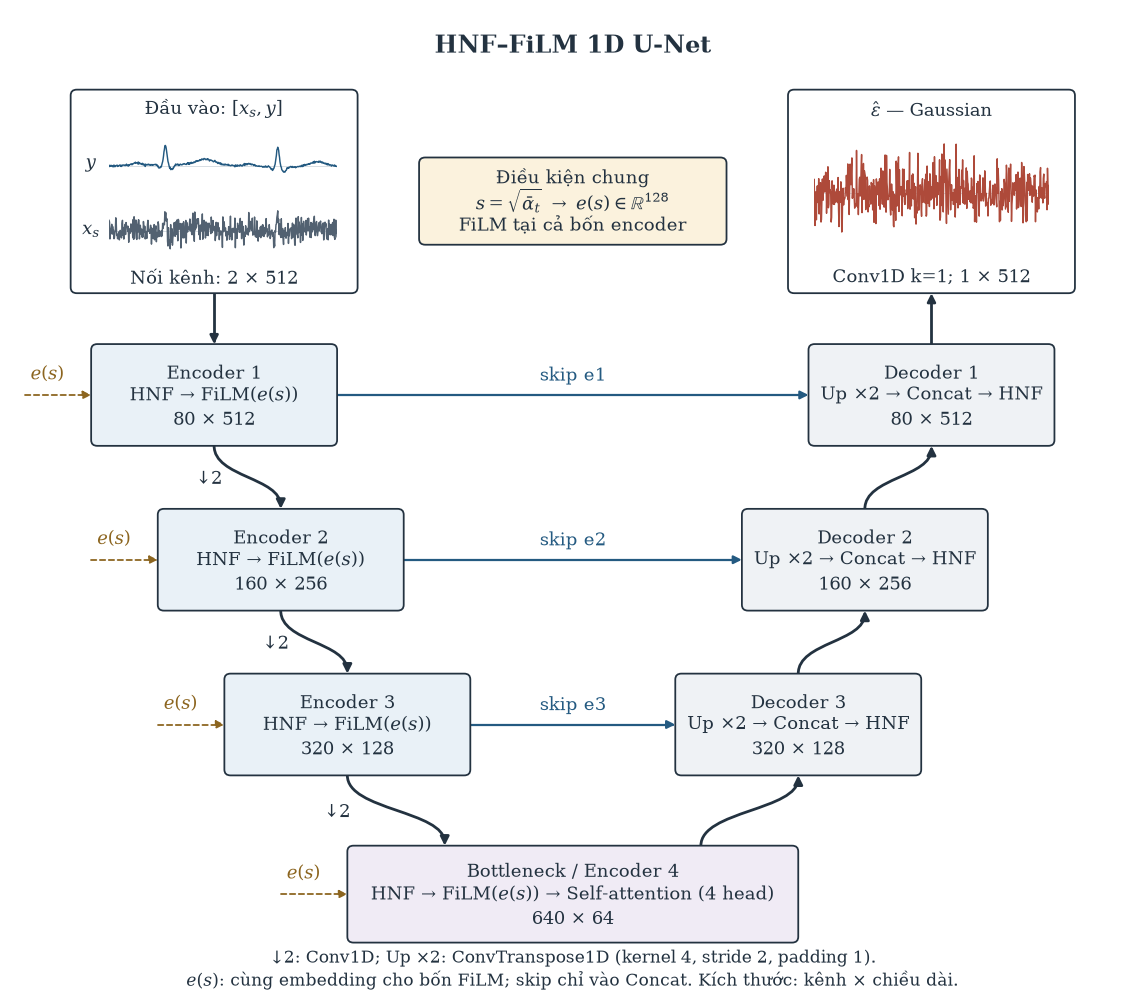
\includegraphics[width=\textwidth,height=0.80\textheight,keepaspectratio]{2.png}
 \caption{Kiến trúc HNF--FiLM 1D U-Net (U4) cho đoạn 512 điểm. Khối giữa đáy gom Encoder 4 và self-attention; mỗi decoder thực hiện Up $\rightarrow$ Concat $\rightarrow$ HNF. Skip lấy đặc trưng encoder sau FiLM. Các nhãn $e(s)$ chỉ cùng embedding điều kiện cho bốn encoder. Đầu vào gồm ECG quan sát $y$ và trạng thái khuếch tán $x_s$; đầu ra $\hat\epsilon$ là Gaussian dự đoán, không phải ECG sạch. Các waveform tổng hợp chỉ minh họa loại tín hiệu, không phải kết quả thực nghiệm.}
 \label{fig:architecture}
\end{figure*}

\subsubsection{Các khối thành phần của kiến trúc}
Hình~\ref{fig:blocks} mô tả các phép xử lý bên trong HNF, FiLM và self-attention. Các đường nối thể hiện đúng vị trí chuẩn hóa, điều chế affine và tổng hợp đặc trưng trong mã nguồn.
\paragraph{Khối HNF đa tỉ lệ}
HNF (Half Normalized Filter) nhận tensor $h$ và tạo bốn nhánh tích chập có tập kernel $\mathcal{K}=\{3,5,9,15\}$. Mỗi nhánh sinh $C_o/4$ kênh, với $C_o$ là số kênh đầu ra của khối. Các nhánh giữ nguyên chiều dài bằng reflection padding. Sau phép nối, tích chập kernel 1 tổng hợp thông tin:
\begin{equation}
 z=\Conv_1\!\left(\Concat_{k\in\mathcal{K}}\Conv_k(h)\right).
 \label{eq:multiscale}
\end{equation}
Chia $z$ thành hai nhóm kênh bằng nhau, $z_a$ và $z_b$. Chỉ $z_a$ được chuẩn hóa theo từng mẫu và từng kênh dọc trục thời gian:
\begin{equation}
 \IN(z_a)_{c,\ell}=\frac{z_{a,c,\ell}-\mu_c}{\sqrt{v_c+\delta}},
 \label{eq:in}
\end{equation}
trong đó $\mu_c$ và $v_c$ là trung bình và phương sai trên chiều thời gian; $\delta>0$ bảo đảm ổn định số. Khối hiện tại không dùng tham số affine học được trong instance normalization. Đầu ra HNF là
\begin{equation}
 \mathcal{H}(h)=\ReLU\!\left(\Concat(\IN(z_a),z_b)\right)+\mathcal{R}(h),
 \label{eq:hnf}
\end{equation}
với $\mathcal{R}$ là Identity nếu số kênh không đổi và Conv1D kernel 1 nếu cần đổi số kênh. Thiết kế phối hợp các trường tiếp nhận cục bộ khác nhau và duy trì một nhánh đặc trưng không đi qua chuẩn hóa. Mức độ bảo toàn biên độ và hình thái phải được xác nhận bằng thực nghiệm, vì tích chập và kích hoạt vẫn biến đổi đặc trưng.

\paragraph{Điều kiện hóa bằng FiLM}
Mức $s$ được biểu diễn bằng embedding hình sin 128 chiều. Với $m=64$ và $j=0,\ldots,m-1$:
\begin{equation}
 \begin{aligned}
 \omega_j&=10000^{-j/(m-1)},\\
 e(s)&=[\sin(s\omega_0),\ldots,\sin(s\omega_{m-1}),\\
     &\hspace{8mm}\cos(s\omega_0),\ldots,\cos(s\omega_{m-1})].
 \end{aligned}
\end{equation}
Ở mỗi mức encoder, phép chiếu tuyến tính và SiLU tạo hai vector theo kênh:
\begin{equation}
 [\gamma_l(s),\xi_l(s)]=\SiLU(W_l e(s)+b_l).
\end{equation}
Phép điều chế là
\begin{equation}
 \mathcal{F}_l(h,s)=h\odot[1+\gamma_l(s)]+\xi_l(s),
 \label{eq:film}
\end{equation}
trong đó các vector được broadcast trên chiều thời gian. FiLM điều chỉnh cả độ khuếch đại và độ dịch của từng kênh theo mức diffusion. ECG quan sát được đưa vào bằng phép nối tín hiệu, còn $s$ được đưa vào qua FiLM; hai nguồn điều kiện này có vai trò khác nhau.

\paragraph{Self-attention tại bottleneck}
Với $e_4$ dài $L_b=L/8$, các tích chập kernel 1 tạo query, key và value. Ở mỗi head, biểu diễn được sắp theo chiều thời gian với $Q_h,K_h,V_h\in\mathbb{R}^{L_b\times d_h}$. Attention được tính bởi
\begin{equation}
 A_h=\softmax\!\left(\frac{Q_h K_h^{\mathsf{T}}}{\sqrt{d_h}}\right),
 \qquad O_h=A_hV_h.
\end{equation}
Kết quả được nối và chiếu về số kênh ban đầu:
\begin{equation}
 \mathcal{A}(e_4)=\Conv_1\!\left(\Concat_{h=1}^{H}O_h\right),
 \label{eq:attention}
\end{equation}
với $H=4$ và $d_h=160$ ở cấu hình $C=80$. Đặt attention ở bottleneck giảm độ dài chuỗi từ $L$ xuống $L/8$, giảm kích thước ma trận tương tác so với đặt ở đầu vào. Phạm vi tương tác giới hạn trong đoạn ECG được đưa vào mạng. Khối attention hiện tại không có lớp chuẩn hóa, dropout hoặc phép cộng residual riêng bên ngoài~\eqref{eq:attention}.

\begin{figure*}[t]
 \centering
 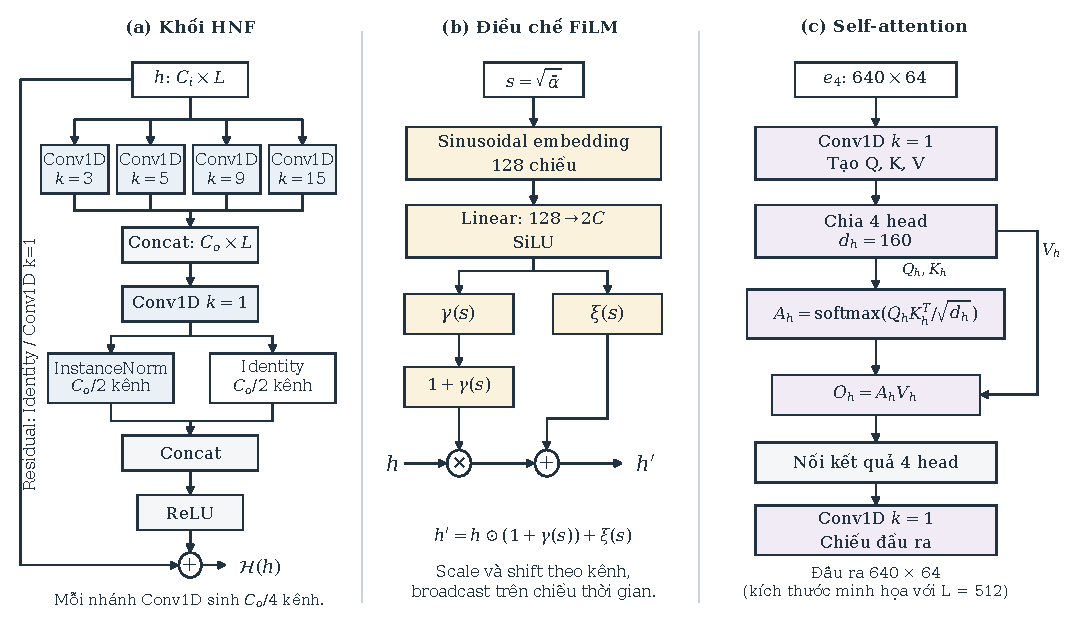
\includegraphics[width=\textwidth]{fig03_blocks.pdf}
 \caption{Các khối thành phần: (a) HNF tổng hợp bốn nhánh kernel, chuẩn hóa một nửa số kênh và cộng residual sau ReLU; (b) FiLM sinh scale và shift từ embedding mức diffusion rồi broadcast trên chiều thời gian; (c) self-attention bốn head với nhánh value và phép chiếu đầu ra. Kích thước ở (c) tương ứng bottleneck của đoạn 512 điểm.}
 \label{fig:blocks}
\end{figure*}

\subsection{Hàm mục tiêu thời gian--tần số}
Thành phần dự đoán nhiễu dùng L1 trung bình:
\begin{equation}
 \mathcal{L}_{\epsilon}=\mathbb{E}_{x_0,y,s,\epsilon}
 \left[\frac{1}{L}\sum_{\ell=1}^{L}|\epsilon_\ell-\hat\epsilon_\ell|\right].
 \label{eq:timeloss}
\end{equation}
Ở đây, ``miền thời gian'' chỉ sai số trên chuỗi nhiễu dự đoán; đây không phải L1 trực tiếp giữa ECG $x_0$ và $\hat x_0$. Lấy trung bình giúp thang đo loss không tăng tuyến tính theo batch size hoặc chiều dài đoạn.

Đặt $M(x)=|\STFT(x)|$. STFT sử dụng cửa sổ Hann, kích thước FFT 128, bước dịch 64; biên được mở rộng phản xạ theo chế độ centered STFT. Với $P$ là số phần tử phổ, sai số tương đối cho một mẫu là
\begin{equation}
 r_f=\frac{\frac{1}{P}\|M(\hat x_0)-M(x_0)\|_F^2}
 {\max\!\left(\frac{1}{P}\|M(x_0)\|_F^2,\delta_f\right)},
 \label{eq:relative}
\end{equation}
trong đó $\delta_f=10^{-6}$. Chuẩn hóa theo năng lượng phổ tham chiếu giúp giảm sự chi phối của những mẫu biên độ lớn.

Ở mức diffusion có $s$ nhỏ, sai số $\Delta\epsilon=\hat\epsilon-\epsilon$ bị khuếch đại khi tái tạo:
\begin{equation}
 \hat x_0-x_0=-\frac{\sqrt{1-s^2}}{s}\,\Delta\epsilon.
\end{equation}
Vì vậy, thành phần phổ được đặt trọng số theo diffusion SNR:
\begin{equation}
 w(s)=\min\!\left(\frac{s^2}{\max(1-s^2,10^{-6})},1\right),
 \quad\mathcal{L}_f=\mathbb{E}[w(s)r_f].
 \label{eq:weight}
\end{equation}
Diffusion SNR khác với SNR của artifact trong ECG quan sát. Mục tiêu tổng là
\begin{equation}
 \mathcal{L}=\lambda_{\epsilon}\mathcal{L}_{\epsilon}+\lambda_f\mathcal{L}_f,
 \quad\lambda_{\epsilon}=1,\quad\lambda_f=0.1.
 \label{eq:total}
\end{equation}
Loss biên độ STFT không ràng buộc trực tiếp pha hoặc từng mốc sinh lý. Nó bổ sung cho sai số dự đoán nhiễu thay vì thay thế toàn bộ mục tiêu học. Trong ablation kiến trúc, toàn bộ loss được giữ cố định để khảo sát ảnh hưởng của HNF, FiLM và attention. Đóng góp độc lập của loss cần nhóm ablation riêng.

\subsection{Suy luận bằng DDIM}
Quy trình suy luận được tóm tắt trong Hình~\ref{fig:system-inference}. DDIM\cite{ddim} sử dụng các mốc $\tau_0=0,\ldots,\tau_S=T$ để cập nhật trạng thái. Tại cặp mốc $t=\tau_j$ và $t'=\tau_{j-1}$, đặt
\begin{equation}
 \begin{aligned}
 \hat\epsilon_t&=\epsilon_\theta(x_t,y,\sqrt{\bar\alpha_t}),\\
 \hat x_0^{(t)}&=\frac{x_t-\sqrt{1-\bar\alpha_t}\hat\epsilon_t}
                         {\sqrt{\bar\alpha_t}},\\
 \sigma_{t,t'}&=\eta\sqrt{\frac{1-\bar\alpha_{t'}}{1-\bar\alpha_t}}
                  \sqrt{1-\frac{\bar\alpha_t}{\bar\alpha_{t'}}}.
 \end{aligned}
\end{equation}
Trạng thái tiếp theo là
\begin{equation}
 \begin{aligned}
 x_{t'}={}&\sqrt{\bar\alpha_{t'}}\hat x_0^{(t)}
       +\sqrt{1-\bar\alpha_{t'}-\sigma_{t,t'}^2}\hat\epsilon_t\\
       &+\sigma_{t,t'}z,\qquad z\sim\mathcal{N}(0,I).
 \end{aligned}
 \label{eq:ddim}
\end{equation}
Tại mốc cuối $t'=0$, đặt $\bar\alpha_0=1$ và $\sigma_{t,0}=0$. Khi $\eta=0$, cập nhật là xác định với $x_T$ cố định; kết quả vẫn phụ thuộc Gaussian khởi tạo. Một lần lấy mẫu (1-shot) là mốc so sánh; lấy trung bình nhiều lần lấy mẫu cần báo cáo riêng cùng chi phí tương ứng.

Notebook hiện sử dụng lịch bậc hai $\tau_j=\lfloor T(j/S)^2\rfloor$. Phép lấy phần nguyên có thể tạo mốc lặp; mốc lặp không tạo bước tiến thời gian mới dù mã nguồn vẫn có thể gọi mạng. Khi khảo sát tốc độ cần công bố số lần đánh giá mạng thực tế (NFE), lịch mốc và latency. Việc dùng DDIM hoặc chọn $S=50$ tự nó chưa chứng minh tăng tốc so với DDPM 50 bước.

\section{Thiết lập thực nghiệm}
\subsection{Nguồn dữ liệu và phạm vi giao thức}
Nguồn ECG duy nhất là QT Database (QTDB)\cite{qtdb}. Cơ sở dữ liệu gồm 105 bản ghi hai kênh lấy mẫu ở 250~Hz, có chú giải liên quan đến các thành phần sóng. Nghiên cứu sử dụng một kênh ECG cho mỗi đoạn. BW, EM và MA được lấy từ MIT-BIH Noise Stress Test Database (NSTDB)\cite{nstdb}; EM chỉ chuyển động điện cực, còn MA chỉ artifact do hoạt động cơ.

Thí nghiệm kiến trúc chính dùng đoạn 512 điểm sau tiền xử lý và một mô hình học nhiều tổ hợp nhiễu. Checkpoint chuyên biệt cho từng BW, EM hoặc MA thuộc giao thức khác và không thay thế U4 huấn luyện bằng dữ liệu trộn. Nhánh benchmark 3600 điểm được mô tả riêng ở Mục~\ref{sec:benchmark3600}; chiều dài đó không được dùng để mô tả đầu vào huấn luyện của ablation 512.

\subsection{Tiền xử lý và phân chia dữ liệu}
\subsubsection{Tạo đoạn ECG tham chiếu}
Mỗi bản ghi được đọc ở kênh chỉ số 0. Chú giải \texttt{pu1}, được tạo tự động từ kênh chỉ số 1 của cùng bản ghi, được sử dụng để xác định khởi đầu P và các mốc nhịp trên trục thời gian chung\cite{qtdb}. Các mốc này không được đồng nhất với ranh giới được chuyên gia gán nhãn thủ công. Điểm bắt đầu đoạn đặt trước khởi đầu P khoảng 40~ms. Hai điểm bắt đầu liên tiếp xác định một đoạn ứng viên.

Đoạn được mở rộng phản xạ ở biên trước khi nội suy lại về 360~Hz, sau đó bỏ phần đệm nội suy. Các đoạn không hợp lệ, có nhiều hơn một mốc R, dài hơn 496 điểm sau resample, không hữu hạn hoặc biên độ không đổi được loại bỏ. Với đoạn hợp lệ $u$, giá trị $[u(0)+u(L_u-1)]/2$ được trừ khỏi toàn đoạn để hiệu chỉnh mức biên. Đoạn được đặt trong mảng zero-padding dài 512 từ vị trí chỉ số 16. Do có phần đệm, 512 là kích thước tensor; thời gian sinh lý hữu ích còn phụ thuộc độ dài đoạn trước đệm. Quy trình này không phải cắt cửa sổ cố định 512 điểm trực tiếp từ bản ghi liên tục.

\subsubsection{Tách train, validation và test}
Giao thức dành riêng 14 record cho test: \texttt{sel123}, \texttt{sel233}, \texttt{sel302}, \texttt{sel307}, \texttt{sel820}, \texttt{sel853}, \texttt{sel16420}, \texttt{sel16795}, \texttt{sele0106}, \texttt{sele0121}, \texttt{sel32}, \texttt{sel49}, \texttt{sel14046} và \texttt{sel15814}. Các đoạn từ những record còn lại được trộn bằng seed cố định và chia 70\% cho train, 30\% cho validation. Bảng~\ref{tab:data} dành cho số lượng mẫu thực tế sau kiểm tra.

\begin{table}[t]
 \caption{Thống kê dữ liệu của giao thức 512 điểm}
 \label{tab:data}
 \centering\small
 \begin{tabular}{@{}lcc@{}}
 \toprule
 Tập & Số record & Số đoạn hợp lệ\\
 \midrule
 Train & \pending & \pending\\
 Validation & \pending & \pending\\
 Test & 14 & \pending\\
 \bottomrule
 \end{tabular}
 \par\smallskip\footnotesize Train/validation chia theo đoạn nên có thể dùng chung record. Số lượng được điền từ manifest sau tiền xử lý.
\end{table}

Test độc lập ở mức record với dữ liệu dùng tối ưu và chọn checkpoint. Train và validation không độc lập ở mức record: các đoạn cùng bản ghi có thể xuất hiện ở cả hai tập. Validation vì vậy không được diễn giải như phép đo tổng quát hóa sang người bệnh hoàn toàn mới. Danh sách split, mã đoạn, tổ hợp nhiễu, cường độ và fingerprint được lưu để U0--U4 dùng cùng dữ liệu.

\subsection{Tạo nhiễu hỗn hợp và chuẩn hóa}
Với thứ tự $(\mathrm{BW},\mathrm{EM},\mathrm{MA})$, mỗi đoạn được gán mask $m\in\{0,1\}^3\setminus\{(0,0,0)\}$. Bảy mask tương ứng BW, EM, MA, BW+EM, BW+MA, EM+MA và BW+EM+MA. Số mask được cân bằng gần đều trên toàn bộ tập đoạn rồi hoán vị bằng seed cố định; tỷ lệ trong từng split có thể khác nhẹ. Cặp dữ liệu được giữ cố định qua các epoch và giữa các biến thể.

Với các patch dài 512 điểm:
\begin{equation}
 \begin{aligned}
 n_{\mathrm{mix}}&=m_1n_{\mathrm{BW}}+m_2n_{\mathrm{EM}}+m_3n_{\mathrm{MA}},\\
 \kappa&=r\,\frac{\operatorname{ptp}(x_0)}{\operatorname{ptp}(n_{\mathrm{mix}})},\\
 r&\in\{0.20,0.21,\ldots,1.99\},
 \end{aligned}
 \label{eq:mix}
\end{equation}
trong đó $\operatorname{ptp}(u)=\max(u)-\min(u)$. Các thành phần được cộng trước rồi mới scale hỗn hợp một lần; quy trình không ép từng nguồn có cùng năng lượng. $r$ là tỷ lệ peak-to-peak, không phải SNR theo dB. Trường hợp peak-to-peak bằng 0 bị báo lỗi.

Ở protocol~1 mặc định, train và validation lấy patch từ nửa đầu theo thời gian, kênh chỉ số 0 của mỗi record NSTDB. Vị trí patch được gán xác định theo chỉ số đoạn. Hai tập có thể tái sử dụng patch; đây không phải phép tách độc lập nguồn nhiễu ở validation. Vùng nhiễu test cần được khóa riêng cùng danh sách patch và seed trước đánh giá. \draftnote{vùng thời gian, kênh và số cặp test của pipeline đánh giá cuối.}

Trong notebook huấn luyện hiện tại, mỗi cặp được chia cùng hệ số
\begin{equation}
 a_i=\max(\|x_{0,i}\|_{\infty},10^{-8}),\quad
 x'_{0,i}=x_{0,i}/a_i,\quad y'_i=y_i/a_i.
 \label{eq:normalization}
\end{equation}
Các công thức phương pháp được áp dụng trong miền đã chuẩn hóa. Đây là chuẩn hóa có tham chiếu trong thí nghiệm cặp sạch--nhiễu; ECG sạch không có sẵn khi triển khai thực tế. Do đó, không thể mặc nhiên xem~\eqref{eq:normalization} là bước suy luận không cần tham chiếu. Giao thức benchmark dùng scale từ noisy input phải công bố riêng; chuyển quy tắc chuẩn hóa cần kiểm chứng sai khác phân phối. Metric được tính trong cùng thang biên độ của từng giao thức và sau hoàn nguyên scale nếu giao thức yêu cầu.

\subsection{Cấu hình và quy trình huấn luyện}
Adam cập nhật tham số từ loss~\eqref{eq:total}, với clipping norm gradient ở 1.0. Sau mỗi cập nhật, trung bình trượt tham số là
\begin{equation}
 \theta^{\mathrm{EMA}}_k=\rho\theta^{\mathrm{EMA}}_{k-1}+(1-\rho)\theta_k,
 \qquad\rho=0.9.
\end{equation}
Notebook dùng StepLR chu kỳ 150 epoch, hệ số 0.1; với ngân sách 100 epoch, learning rate không giảm. DataLoader dùng \texttt{drop\_last=True} cho train và validation; số đoạn được duyệt ở mỗi tập là $B\lfloor N/B\rfloor$. Cần phân biệt số đoạn được chuẩn bị với số đoạn thực tế tính loss trong một epoch.

\begin{table}[t]
 \caption{Cấu hình huấn luyện của thí nghiệm kiến trúc 512}
 \label{tab:config}
 \centering\small
 \begin{tabular}{@{}ll@{}}
 \toprule
 Tham số & Giá trị\\
 \midrule
 Kênh ECG / chiều dài tensor & 1 / 512 điểm\\
 Tần số sau resample & 360~Hz\\
 Kênh vào / ra mạng & 2 / 1\\
 Số kênh encoder & 80, 160, 320, 640\\
 Embedding / head attention & 128 / 4\\
 Diffusion steps $T$ & 50\\
 $\beta_{\min}$ / $\beta_{\max}$ & $10^{-4}$ / $0.5$\\
 Lịch $\beta$ & Bậc hai\\
 Optimizer / learning rate & Adam / $10^{-4}$\\
 Batch size / epoch & 96 / 100\\
 $\lambda_{\epsilon}$ / $\lambda_f$ & 1 / 0.1\\
 FFT / bước dịch STFT & 128 / 64\\
 EMA / clipping norm & 0.9 / 1.0\\
 Seed dữ liệu và huấn luyện & 1234\\
 GPU / phiên bản thư viện & \pending\\
 \bottomrule
 \end{tabular}
\end{table}

Validation chạy sau mỗi epoch với trạng thái ngẫu nhiên cố định, giảm biến động do lấy mẫu timestep và Gaussian. Checkpoint tốt nhất được chọn theo validation loss của mạng hiện hành, không phải metric test hoặc validation của EMA. Checkpoint lưu mạng hiện hành và EMA tại epoch được chọn, cùng optimizer, scheduler, trạng thái RNG và fingerprint. Nếu dùng EMA khi đánh giá, cần nạp EMA đúng checkpoint đó và áp dụng nhất quán cho mọi biến thể. Luồng huấn luyện và chọn checkpoint được tóm tắt trong Hình~\ref{fig:system-training}.

\begin{figure}[t]
 \centering
 \begin{minipage}{\linewidth}
 \small
 \begin{algorithmic}[1]
 \REQUIRE Các cặp $(x_0,y)$, lịch $\beta$, tham số $\theta$
 \FOR{mỗi epoch}
   \FOR{mỗi mini-batch huấn luyện}
     \STATE Chọn $t$, lấy mức $s$ và Gaussian $\epsilon$
     \STATE Tạo $x_s$ theo~\eqref{eq:continuous}
     \STATE Dự đoán $\hat\epsilon=\epsilon_\theta(x_s,y,s)$
     \STATE Tái tạo $\hat x_0$ theo~\eqref{eq:x0}
     \STATE Tính $\mathcal{L}_{\epsilon}$, $\mathcal{L}_f$ và $\mathcal{L}$
     \STATE Lan truyền ngược, clip gradient, cập nhật Adam
     \STATE Cập nhật $\theta^{\mathrm{EMA}}$
   \ENDFOR
   \STATE Tính validation loss với seed cố định
   \STATE Lưu checkpoint cuối; cập nhật checkpoint tốt nhất
 \ENDFOR
 \ENSURE Checkpoint được chọn bằng validation và EMA tương ứng
 \end{algorithmic}
 \end{minipage}
 \caption{Quy trình huấn luyện conditional DDPM với loss đa miền.}
 \label{fig:algorithm}
\end{figure}

\subsection{Thiết kế ablation kiến trúc}
U0 là conditional diffusion U-Net cơ sở dùng hai Conv1D kernel 3 với ReLU trong mỗi khối đặc trưng. U0 vẫn nhận $x_s$, $y$ và $s$; mức diffusion được đưa vào bằng phép cộng embedding đã chiếu:
\begin{equation}
 \mathcal{F}_{\mathrm{add}}(h,s)=h+\SiLU(W e(s)+b).
\end{equation}
Khi bỏ HNF, Conv1D thay thế giữ nguyên số kênh vào/ra và chiều dài feature. Khi bỏ attention, khối tương ứng là Identity. Bảng~\ref{tab:ablation} cho biết các tổ hợp; tất cả dùng cùng dữ liệu trộn, diffusion, loss, optimizer và số epoch.

\begin{table}[t]
 \caption{Các biến thể kiểm chứng thành phần kiến trúc}
 \label{tab:ablation}
 \centering\small
 \begin{tabular}{@{}lcccc@{}}
 \toprule
 Mạng & Đặc trưng & Mức diffusion & Attn & Tham số (M)\\
 \midrule
 U0 & Conv1D & Cộng embedding & Không & 6.765\\
 U1 & HNF & Cộng embedding & Không & 9.711\\
 U2 & Conv1D & FiLM & Không & 6.920\\
 U3 & HNF & FiLM & Không & 9.866\\
 U4 & HNF & FiLM & Có & 11.507\\
 \bottomrule
 \end{tabular}
\end{table}

U1--U0 khảo sát thay Conv1D bằng HNF; U2--U0 khảo sát FiLM trên khung Conv1D; U3--U1 khảo sát FiLM khi có HNF; U4--U3 khảo sát self-attention. U3--U2 bổ sung đối chiếu HNF khi dùng FiLM. Đây là ablation có kiểm soát cấu hình nhưng không khớp số tham số: thay khối đồng thời thay đổi dung lượng và các phép xử lý bên trong. Kết quả không tách riêng tác động của đa tỉ lệ, half normalization và residual trong HNF.

\subsection{Chỉ số và quy trình đánh giá}
Với đoạn tham chiếu $x$, đầu vào $y$, dự đoán $\hat x$ và $e=x-\hat x$, metric được tính từng đoạn trước khi tổng hợp:
\begin{equation}
 \begin{aligned}
 \mathrm{SSD}&=\sum_{\ell=1}^{L}e_\ell^2,\\
 \mathrm{RMSE}&=\sqrt{\frac{1}{L}\sum_{\ell=1}^{L}e_\ell^2},\\
 \mathrm{MAD}&=\max_{\ell}|e_\ell|.
 \end{aligned}
\end{equation}
MAD ở đây là sai khác tuyệt đối lớn nhất, không phải trung bình. PRD theo năng lượng tín hiệu và độ tương đồng cosine là
\begin{equation}
 \mathrm{PRD}_{E}=100\sqrt{\frac{\sum_\ell e_\ell^2}{\sum_\ell x_\ell^2}},
 \label{eq:prd}
\end{equation}
\begin{equation}
 \mathrm{CosSim}=\frac{\sum_\ell x_\ell\hat x_\ell}
 {\sqrt{\sum_\ell x_\ell^2}\sqrt{\sum_\ell\hat x_\ell^2}}.
\end{equation}
Mẫu năng lượng bằng 0 được phát hiện trong kiểm tra dữ liệu hoặc xử lý bằng hằng số ổn định thống nhất. Một số benchmark dùng mẫu số PRD khác, như năng lượng đã trừ trung bình hoặc đại lượng dựa trên prediction; các biến thể đó phải ghi tên riêng và không thay thế trực tiếp cho~\eqref{eq:prd}.

SNR đầu ra và mức cải thiện là
\begin{equation}
 \begin{aligned}
 \mathrm{SNR}_{\mathrm{out}}&=10\log_{10}
    \frac{\sum_\ell x_\ell^2}{\sum_\ell (x_\ell-\hat x_\ell)^2},\\
 \mathrm{SNR}_{\mathrm{in}}&=10\log_{10}
    \frac{\sum_\ell x_\ell^2}{\sum_\ell (x_\ell-y_\ell)^2},\\
 \Delta\mathrm{SNR}&=\mathrm{SNR}_{\mathrm{out}}-\mathrm{SNR}_{\mathrm{in}}.
 \end{aligned}
\end{equation}
SSD, RMSE, MAD và PRD càng thấp càng tốt; SNR càng cao và CosSim càng gần 1 càng tốt. CosSim không phản ánh đầy đủ sai lệch biên độ nên được xem cùng các metric sai số.

Các mô hình nhận cùng noisy test, thứ tự mã mẫu và thang biên độ. Trung bình và độ lệch chuẩn tính từ metric từng đoạn; có thể bổ sung tổng hợp theo record để phản ánh sự phụ thuộc giữa các đoạn cùng bản ghi. Phân tích theo nhóm nhiễu sử dụng một checkpoint hỗn hợp của mỗi biến thể. So sánh checkpoint chuyên biệt hoặc nhiễu chưa thấy được khai báo là thí nghiệm riêng.

Latency được đo sau warm-up, đồng bộ GPU trước và sau suy luận, với cùng phần cứng và batch size. Báo cáo cần ghi số shot, NFE và có bao gồm tiền xử lý hay không. Với batch $B_{\mathrm{eval}}$ có thời gian $t_{\mathrm{batch}}$, thời gian mỗi đoạn là $t_{\mathrm{batch}}/B_{\mathrm{eval}}$. \draftnote{seed khởi tạo suy luận, batch đánh giá, cấu hình DDIM và số lần đo cuối.}

\section{Kết quả và thảo luận}
% TODO-RESULTS: Chi ket luan sau khi can sample_id, metric, normalization.
\subsection{Chất lượng phục hồi trên dữ liệu kiểm thử chung}
Bảng~\ref{tab:mainresults} dành cho kết quả chính trên giao thức 512. Mỗi hàng sử dụng cùng tập test và định nghĩa metric. Baseline được đưa vào sau khi chạy lại hoặc xác nhận đầy đủ tính tương thích giao thức. So sánh U4 với U0 đánh giá tác động tổng hợp của các thành phần kiến trúc trong cùng khung conditional diffusion.

\begin{table*}[t]
 \caption{Kết quả trên giao thức QTDB 512 điểm, trình bày theo trung bình $\pm$ độ lệch chuẩn}
 \label{tab:mainresults}
 \centering\small
 \begin{tabular}{@{}lccccccc@{}}
 \toprule
 Phương pháp & SSD $\downarrow$ & MAD $\downarrow$ & RMSE $\downarrow$ & PRD$_E$ (\%) $\downarrow$ & CosSim $\uparrow$ & SNR$_{\mathrm{out}}$ (dB) $\uparrow$ & $\Delta$SNR (dB) $\uparrow$\\
 \midrule
 ECG đầu vào & \pending & \pending & \pending & \pending & \pending & \pending & 0\\
 Bộ lọc truyền thống: \draftnote{tên} & \pending & \pending & \pending & \pending & \pending & \pending & \pending\\
 Mô hình đối chứng: \draftnote{tên} & \pending & \pending & \pending & \pending & \pending & \pending & \pending\\
 U0: diffusion U-Net cơ sở & \pending & \pending & \pending & \pending & \pending & \pending & \pending\\
 U4: mô hình đề xuất & \pending & \pending & \pending & \pending & \pending & \pending & \pending\\
 \bottomrule
 \end{tabular}
\end{table*}

\draftnote{số đoạn test, SNR đầu vào, kết quả từng phương pháp và chênh lệch thực nghiệm.} Phân tích cần xét cả sai số biên độ và tương đồng dạng sóng. SSD tăng theo chiều dài và thang biên độ, do đó không đối chiếu trực tiếp trị tuyệt đối SSD giữa đoạn 512 và 3600.

\subsection{Đóng góp của các thành phần kiến trúc}
Bảng~\ref{tab:ablationresults} dành cho kết quả U0--U4. Đối chiếu được thực hiện theo từng cặp đã nêu, thay vì suy luận vai trò một khối từ hai hệ thống khác hoàn toàn. Nếu hiệu quả một khối phụ thuộc nhóm nhiễu hoặc metric, cần chỉ rõ điều kiện đó.

\begin{table}[t]
 \caption{Ablation kiến trúc trên cùng tập test 512}
 \label{tab:ablationresults}
 \centering\small
 \begin{tabular}{@{}lcccc@{}}
 \toprule
 Mạng & RMSE $\downarrow$ & PRD$_E$ $\downarrow$ & $\Delta$SNR $\uparrow$ & ms/đoạn $\downarrow$\\
 \midrule
 U0 & \pending & \pending & \pending & \pending\\
 U1 & \pending & \pending & \pending & \pending\\
 U2 & \pending & \pending & \pending & \pending\\
 U3 & \pending & \pending & \pending & \pending\\
 U4 & \pending & \pending & \pending & \pending\\
 \bottomrule
 \end{tabular}
\end{table}

\draftnote{nhận định U1--U0, U2--U0, U3--U1, U3--U2 và U4--U3 từ số liệu.} Mức tăng tham số và thời gian cần được xem cùng chất lượng phục hồi. Nhóm ablation này chưa đủ kết luận riêng về hiệu quả của STFT hoặc trọng số diffusion SNR.

\subsection{Phân tích theo tổ hợp nhiễu và dạng sóng}
Bảng~\ref{tab:noises} trình bày khả năng xử lý các nhóm nhiễu bằng cùng checkpoint U4. Các nhóm đã xuất hiện trong phân phối huấn luyện, nên kết quả phản ánh khả năng làm việc trên mẫu mới của những loại nhiễu đã học. Để kiểm chứng loại nhiễu hoàn toàn chưa thấy cần thiết kế leave-one-noise-type-out hoặc đánh giá ngoài phân phối.

\begin{table}[t]
 \caption{Kết quả U4 theo nhóm nhiễu trên tập test}
 \label{tab:noises}
 \centering\small
 \begin{tabular}{@{}lcccc@{}}
 \toprule
 Nhóm & $N$ & RMSE & PRD$_E$ (\%) & $\Delta$SNR (dB)\\
 \midrule
 BW & \pending & \pending & \pending & \pending\\
 EM & \pending & \pending & \pending & \pending\\
 MA & \pending & \pending & \pending & \pending\\
 BW+EM & \pending & \pending & \pending & \pending\\
 BW+MA & \pending & \pending & \pending & \pending\\
 EM+MA & \pending & \pending & \pending & \pending\\
 BW+EM+MA & \pending & \pending & \pending & \pending\\
 \bottomrule
 \end{tabular}
\end{table}

Hình~\ref{fig:waveforms} dành cho các đoạn đại diện với cùng trục thời gian và thang biên độ giữa ECG tham chiếu, đầu vào và đầu ra. Cần ghi mã record, mã đoạn, loại nhiễu và SNR đầu vào; chọn ví dụ theo tiêu chí công bố, có cả trường hợp điển hình và sai số lớn. Quan sát vùng P, QRS và T giúp mô tả vị trí sai lệch nhưng không thay thế đánh giá định lượng từng thành phần sóng.

\begin{figure*}[t]
 \centering
 \figplaceholder{38mm}{Hình tín hiệu sẽ bổ sung\\ECG tham chiếu / ECG nhiễu / ECG phục hồi / sai số\\Ví dụ có mã mẫu và cùng thang biên độ; phóng to vùng cần phân tích}
 \caption{Ví dụ phục hồi ECG trên các nhóm nhiễu. Mỗi đồ thị cần thể hiện trục thời gian, đơn vị biên độ và thông tin mẫu.}
 \label{fig:waveforms}
\end{figure*}

\subsection{Đánh đổi chất lượng và chi phí suy luận}
Bảng~\ref{tab:ddimresults} dành cho khảo sát sampler với cùng checkpoint. Các mức $S$ là cấu hình khảo sát, chưa phải kết quả đã thực hiện khi chưa có số đo. Cấu hình báo cáo chính cần được chọn trên validation hoặc theo quy tắc định trước, tránh tối ưu số bước và seed trực tiếp trên test.

\begin{table}[t]
 \caption{Khảo sát sampler với cùng checkpoint và phần cứng}
 \label{tab:ddimresults}
 \centering\small
 \begin{tabular}{@{}lccccc@{}}
 \toprule
 Sampler & $S$ & Shot & NFE & RMSE & ms/đoạn\\
 \midrule
 DDPM & 50 & 1 & \pending & \pending & \pending\\
 DDIM, $\eta=0$ & 10 & 1 & \pending & \pending & \pending\\
 DDIM, $\eta=0$ & 25 & 1 & \pending & \pending & \pending\\
 DDIM, $\eta=0$ & 50 & 1 & \pending & \pending & \pending\\
 \bottomrule
 \end{tabular}
\end{table}

\draftnote{đường cong train/validation, độ ổn định hội tụ và phân tích chất lượng--latency.} Chỉ kết luận ``tăng tốc'' khi có số đo trên cùng điều kiện. Với nhiều shot, cải thiện chất lượng cần được đặt cạnh NFE và tổng thời gian tăng thêm.

\subsection{Benchmark bổ sung trên đoạn 3600 điểm}
\label{sec:benchmark3600}
% TODO-BENCHMARK: Bo sung dataset, model, checkpoint va training protocol.
Nhánh benchmark bổ sung sử dụng QTDB dài 3600 điểm để so sánh với các hệ thống bên ngoài. Đây là giao thức riêng về chiều dài, tiền xử lý và nguồn checkpoint. Không mô tả checkpoint huấn luyện riêng ở 3600 là thành viên của ablation 512, hoặc mặc nhiên khẳng định checkpoint 512 đã được kiểm chứng trên 3600. Mạng tích chập cho phép chiều dài chia hết cho 8; khả năng chạy forward không tự chứng minh chất lượng chuyển chiều dài.

Để so sánh trực tiếp, prediction phải khớp mã mẫu, cặp clean--noisy và thang biên độ. Nếu đối chứng dùng checkpoint công khai còn mô hình đề xuất được huấn luyện mới, cần ghi nguồn checkpoint và khác biệt huấn luyện; cùng tập test không đồng nghĩa cùng điều kiện huấn luyện. Số liệu lấy từ bài báo khác chỉ là tham khảo khi chưa xác nhận cùng giao thức. \draftnote{common dataset, danh sách mô hình, checkpoint, chuẩn hóa, sampler và kết quả benchmark 3600.}

\subsection{Giới hạn và hướng mở rộng}
Nghiên cứu sử dụng ECG một kênh và artifact cộng tổng hợp từ NSTDB; kết quả không bao quát mọi thiết bị hoặc điều kiện ghi. Chia train/validation theo đoạn và khả năng dùng chung patch nhiễu hạn chế diễn giải về tính độc lập của validation. Chuẩn hóa tham chiếu ở giao thức 512 cần được chuyển sang quy tắc không phụ thuộc tín hiệu sạch và kiểm chứng lại trước triển khai thực tế.

U0--U4 có số tham số khác nhau, vì vậy cần thận trọng khi quy toàn bộ chênh lệch cho riêng cơ chế một khối. Loss STFT chỉ mô tả biên độ phổ; metric toàn đoạn có thể bỏ sót sai lệch cục bộ. Hướng mở rộng gồm đánh giá theo ranh giới sóng, sai số khoảng thời gian, dữ liệu ngoài QTDB, nhiều seed và tách theo record cho cả train/validation. Chưa có thực nghiệm chẩn đoán sau khử nhiễu nên bài không kết luận về lợi ích lâm sàng trực tiếp.

\section{Kết luận}
Bài báo trình bày phương pháp khử nhiễu ECG một đạo trình bằng conditional DDPM với mạng HNF--FiLM 1D U-Net. Mô hình kết hợp trích xuất đa tỉ lệ, điều chế theo mức khuếch tán và self-attention tại bottleneck; mục tiêu học phối hợp dự đoán nhiễu với sai số phổ tương đối có trọng số. Giao thức dữ liệu trộn BW/EM/MA và bộ biến thể U0--U4 cung cấp cơ sở đánh giá một mô hình trên nhiều nhóm nhiễu và khảo sát đóng góp thành phần. \draftnote{nhận định cuối và chỉ số chính đã xác nhận từ thực nghiệm.} Hướng tiếp theo tập trung vào chuẩn hóa không cần tham chiếu, đánh giá độc lập theo record và giảm chi phí suy luận trong khi duy trì độ chính xác phục hồi.

% Chi can bang cot thu cong sau khi chot toan bo hinh va bang ket qua.
\begin{thebibliography}{99}

\bibitem{chiang2019}
H.-T. Chiang, Y.-Y. Hsieh, S.-W. Fu, K.-H. Hung, Y. Tsao, and S.-Y. Chien, ``Noise reduction in ECG signals using fully convolutional denoising autoencoders,'' \textit{IEEE Access}, vol. 7, pp. 60806--60813, 2019, doi: \href{https://doi.org/10.1109/ACCESS.2019.2912036}{\nolinkurl{10.1109/ACCESS.2019.2912036}}.

\bibitem{nstdb}
G. B. Moody, W. Muldrow, and R. G. Mark, ``MIT-BIH Noise Stress Test Database (version 1.0.0),'' PhysioNet, 1992, doi: \href{https://doi.org/10.13026/C2HS3T}{\nolinkurl{10.13026/C2HS3T}}.

\bibitem{thakor1991}
N. V. Thakor and Y.-S. Zhu, ``Applications of adaptive filtering to ECG analysis: Noise cancellation and arrhythmia detection,'' \textit{IEEE Trans. Biomed. Eng.}, vol. 38, no. 8, pp. 785--794, 1991, doi: \href{https://doi.org/10.1109/10.83591}{\nolinkurl{10.1109/10.83591}}.

\bibitem{deepfilter}
F. P. Romero, D. C. Piñol, and C. R. Vázquez-Seisdedos, ``DeepFilter: An ECG baseline wander removal filter using deep learning techniques,'' arXiv:2101.03423, 2021. [Online]. Available: \url{https://arxiv.org/abs/2101.03423}

\bibitem{fgdae}
A. Shaheen, L. Ye, C. Karunaratne, and T. Seppänen, ``Fully-Gated Denoising Auto-Encoder for Artifact Reduction in ECG Signals,'' \textit{Sensors}, vol. 25, no. 3, Art. no. 801, 2025, doi: \href{https://doi.org/10.3390/s25030801}{\nolinkurl{10.3390/s25030801}}.

\bibitem{ddpm}
J. Ho, A. Jain, and P. Abbeel, ``Denoising diffusion probabilistic models,'' in \textit{Advances in Neural Information Processing Systems}, vol. 33, pp. 6840--6851, 2020.

\bibitem{descod}
H. Li, G. Ditzler, J. Roveda, and A. Li, ``DeScoD-ECG: Deep score-based diffusion model for ECG baseline wander and noise removal,'' \textit{IEEE J. Biomed. Health Inform.}, vol. 28, no. 9, pp. 5081--5091, 2024, doi: \href{https://doi.org/10.1109/JBHI.2023.3237712}{\nolinkurl{10.1109/JBHI.2023.3237712}}.

\bibitem{bwcomparison}
F. P. Romero, L. V. Romaguera, C. R. Vázquez-Seisdedos, C. F. F. C. Filho, M. G. F. Costa, and J. E. Neto, ``Baseline wander removal methods for ECG signals: A comparative study,'' arXiv:1807.11359, 2018. [Online]. Available: \url{https://arxiv.org/abs/1807.11359}

\bibitem{ddim}
J. Song, C. Meng, and S. Ermon, ``Denoising diffusion implicit models,'' in \textit{Proc. Int. Conf. Learning Representations (ICLR)}, 2021. [Online]. Available: \url{https://arxiv.org/abs/2010.02502}

\bibitem{unet}
O. Ronneberger, P. Fischer, and T. Brox, ``U-Net: Convolutional networks for biomedical image segmentation,'' in \textit{Proc. MICCAI}, pp. 234--241, 2015, doi: \href{https://doi.org/10.1007/978-3-319-24574-4_28}{\nolinkurl{10.1007/978-3-319-24574-4_28}}.

\bibitem{hinet}
L. Chen, X. Lu, J. Zhang, X. Chu, and C. Chen, ``HINet: Half instance normalization network for image restoration,'' in \textit{Proc. IEEE/CVF Conf. Computer Vision and Pattern Recognition Workshops}, pp. 182--192, 2021. [Online]. Available: \url{https://arxiv.org/abs/2105.06086}

\bibitem{film}
E. Perez, F. Strub, H. de Vries, V. Dumoulin, and A. Courville, ``FiLM: Visual reasoning with a general conditioning layer,'' in \textit{Proc. AAAI Conf. Artificial Intelligence}, vol. 32, no. 1, 2018. [Online]. Available: \url{https://arxiv.org/abs/1709.07871}

\bibitem{attention}
A. Vaswani \textit{et al.}, ``Attention is all you need,'' in \textit{Advances in Neural Information Processing Systems}, vol. 30, pp. 5998--6008, 2017.

\bibitem{qtdb}
P. Laguna, R. G. Mark, A. L. Goldberger, and G. B. Moody, ``QT Database (version 1.0.0),'' PhysioNet, 1997, doi: \href{https://doi.org/10.13026/C24K53}{\nolinkurl{10.13026/C24K53}}.

\end{thebibliography}

\end{document}
